\documentclass{article}
\usepackage[utf8]{inputenc}

\usepackage{float}
\usepackage{natbib}
\usepackage{graphicx}
\usepackage[export]{adjustbox}
\usepackage{multirow}
\usepackage{hyperref}
\usepackage{titlesec}
\usepackage{ragged2e}



\begin{document}
\title{COS301 Team Gamma: Neural Network Team Goals}
\begin{figure}
    \centering
    
\includegraphics[width=\textwidth]{logo.png}
\end{figure}
\date{March 2020}

\maketitle

\section{Introduction}
This document describes the responsibilities and all deliverables for the \\Neural Network Team.
\\ \\
Demo \#1 Due Date: Thursday 12 March 20:00
\newpage

\section{Organisation}
\subsection{ClickUP}
You need to elect a team leader if you have not done so already. Work together with this member to create tasks and sub-tasks for each member in your team on \url{http://clickup.com} (on the COS301 workspace you have been invited to). \\

\begin{figure}[h]
    \centering
    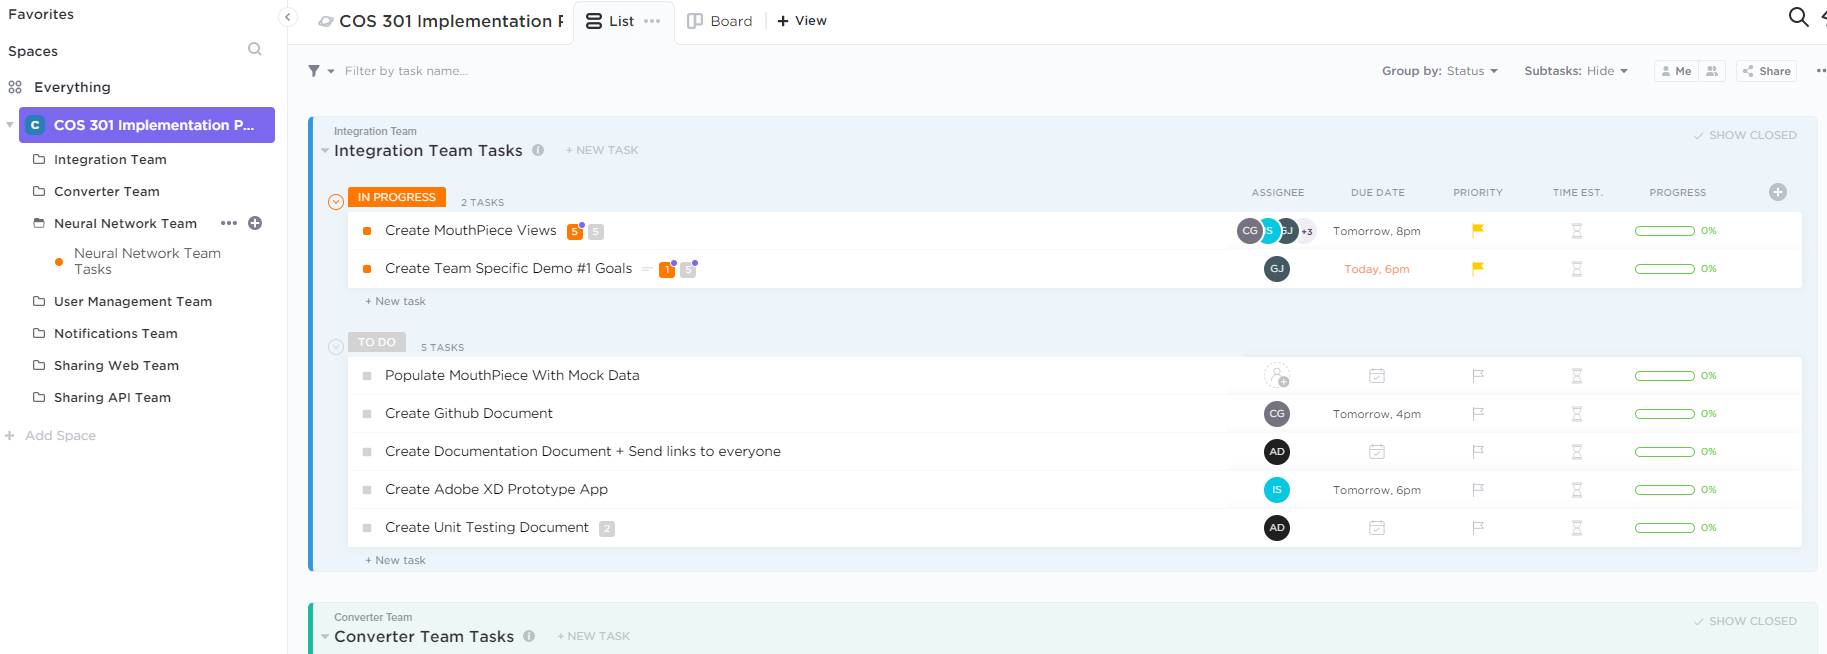
\includegraphics[width=\textwidth]{clickup.png}
\end{figure}

Ensure that you indicate progress and mark tasks as complete. This page will be displayed at the demo.

\subsection{Slack}
Although we have created a WhatsApp group - we do still find it easier for in-group discusions to happen on the slack channels. Simply login to \url{http://cos-301.slack.com}

\newpage

\section{Overall Team Tasks}
These are the tasks to be done by your team for the final product (not specifically Friday's demo).

\begin{itemize}
    \item Deploy a server-side Neural Network
    \item Store a “master” “global” Neural Network model online
    \item Improve this model by adding new training data uploaded by the user
    \item Provide the Converter Team with the trained model
    \item Help the Converter Team to implement and query the model

\end{itemize}

\vspace{1cm}

\begin{center}
   \textit{The tasks are always subject to change, but we have tried our utmost best to sketch out the entire project ahead.}
\end{center}

\newpage


\section{Team Tasks for Friday}

\subsection{Documentation}
\textbf{All documentation to be created in Overleaf} - Overleaf link to be sent to the Integration Team

\subsubsection{Implementation Plan}
Create a document explaining how the neural network will function and integrate with the rest of the system. \\

\textbf{More specifically:}
\begin{itemize}
    \item Explain your plan to train the model and which data the model will give as output
    \item List the technologies that you will use 
    \item Draw basic flow diagrams on \url{http://draw.io} depicting which parts of the Neural Network run where (model on device, training on server) and how that interaction works
    
\end{itemize}

\subsubsection{Frameworks}
You are required to do some research on frameworks that you could implement to assist your \textbf{Overall Team Tasks}. Write a short report on only the frameworks that you are keen to implement. Show its benefits and how you can implement it with the existing technologies. \\

\textbf{Some examples}
\begin{itemize}
    \item \url{https://voice.mozilla.org/}
    \item \url{https://www.tensorflow.org/}
    \item \url{https://pub.dev/packages/ai}
\end{itemize}

\newpage

\subsection{Development Environment}
You are required to setup the development environment (have it running on at least one member's device, ready to demo). Setup everything you think you require. \\
\newline
\textbf{At bear minimum}
\begin{itemize}
    \item Android Studio
    \item Visual Studio Code
    \item Flutter
\end{itemize}

\begin{center}
   \textit{This is required for your implementation in any case.}
\end{center}

\subsection{Hosting Environment}
You will need show the environment where the Neural Network will be hosted and trained.

\subsection{Implementation}
Up to the team to devise a functional demo to showcase the direction they are heading.

\subsubsection{Unit Testing}
Describe how your team will implement unit testing. Better yet - implement it in the Demo where possible.


\end{document}